\documentclass{beamer}
\beamertemplatenavigationsymbolsempty
\usecolortheme{beaver}
\setbeamertemplate{blocks}[rounded=true, shadow=true]
\setbeamertemplate{footline}[page number]
%
\usepackage[utf8]{inputenc}
\usepackage[english,russian]{babel}
\usepackage{amssymb,amsfonts,amsmath,mathtext}
\usepackage{subfig}
\usepackage[all]{xy} % xy package for diagrams
\usepackage{array}
\usepackage{multicol} % many columns in slide
\usepackage{hyperref} % urls
\usepackage{hhline} %tables
\usepackage{comment} %comments
% Your figures are here:
\graphicspath{ {fig/} {../fig/} }

%----------------------------------------------------------------------------------------------------------

\title[\hbox to 56mm{Моделирование динамики физических систем}]{Моделирование динамики физических систем\\ с помощью Physics-Informed Neural Networks}
\author[А.\,И.~Богданов]{Александр Иванович Богданов}
\institute{Московский физико-технический институт}
\date{\footnotesize
\par\smallskip\emph{Курс:} Моя первая научная статья
\par\smallskip\emph{Консультант:} К.\,К.~Панченко
\par\bigskip\small 2023}

%----------------------------------------------------------------------------------------------------------

\begin{document}

%----------------------------------------------------------------------------------------------------------

\begin{frame}

    \thispagestyle{empty}
    \maketitle
    
\end{frame}

%-----------------------------------------------------------------------------------------------------

\begin{comment}
\begin{frame}{Цель исследования}
%\begin{block}{Решается задача}
%\end{block}
\end{frame}
\end{comment}

%-----------------------------------------------------------------------------------------------------

\begin{frame}{Моделирование физической системы}

    $$\frac{d}{dt} \frac{\partial L}{\partial \dot{q}} - \frac{\partial L}{\partial q} = Q^n$$
    
    $$\mathbf{\ddot{q}} = \left( \nabla_{\dot{\mathbf{q}} \dot{\mathbf{q}}} L\right)^{-1} \left[ \nabla_{q} L + Q - \left( \nabla_{\dot{\mathbf{q}} \mathbf{q}} L \right) \dot{\mathbf{q}} \right]$$

    \bigskip

    \begin{columns}[c]

        \column{0.5\textwidth}
            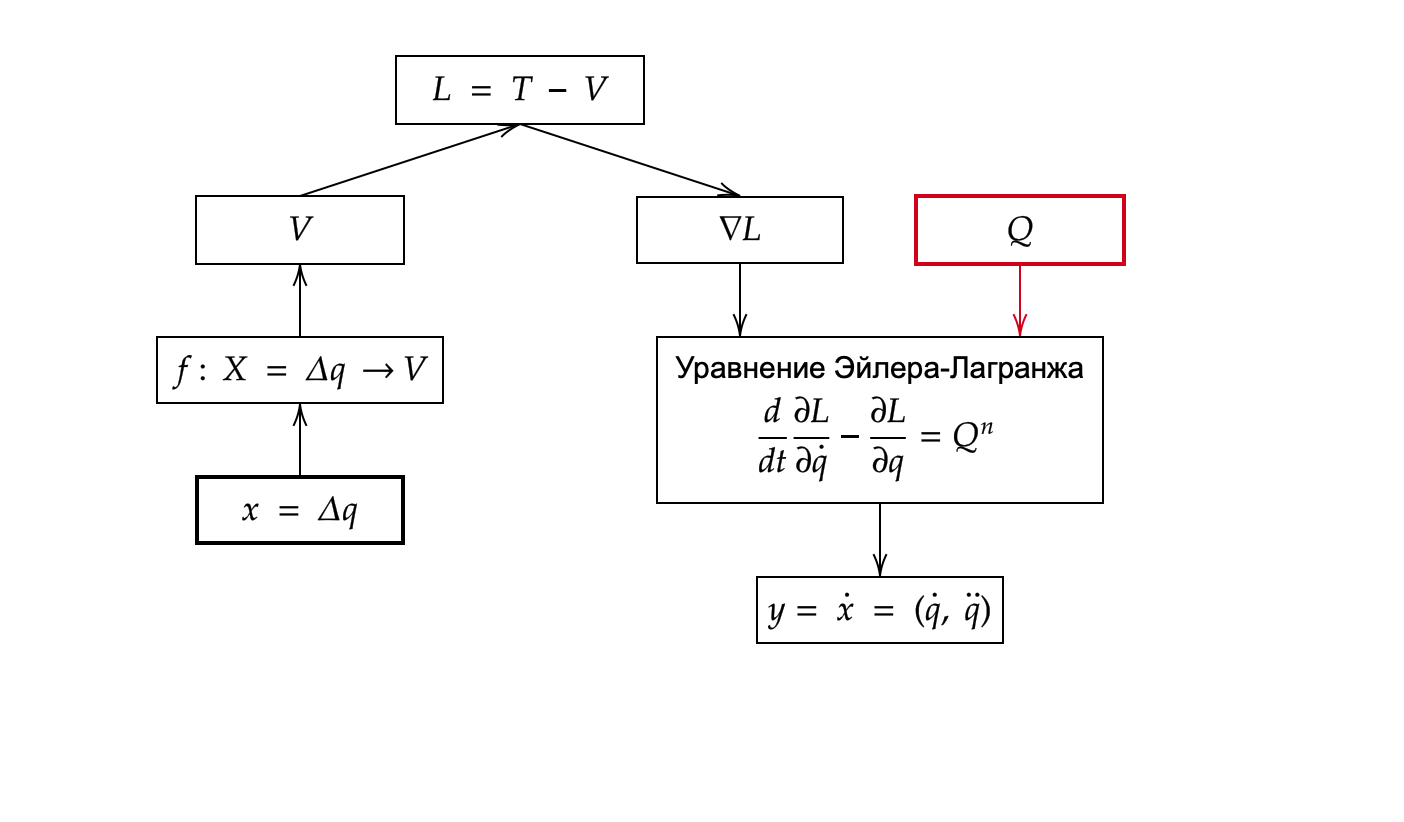
\includegraphics[width=1.4\textwidth]{Diagram}

        \column{0.5\textwidth}
            \includegraphics[width=0.9\textwidth]{Trajectory} 
            
    \end{columns}

\end{frame}

\begin{comment}
%----------------------------------------------------------------------------------------------------------
\begin{frame}{Постановка задачи}

\end{frame}
%----------------------------------------------------------------------------------------------------------
\begin{frame}{Решение}
\begin{columns}[c]
\column{0.6\textwidth}
    Столбец 1
\column{0.4\textwidth}
    Столбец 2
\end{columns}
\end{frame}
%----------------------------------------------------------------------------------------------------------
\begin{frame}{Вычислительный эксперимент}

\end{frame}
%----------------------------------------------------------------------------------------------------------
\begin{frame}{Заключение}
    \begin{block}{Перечислите ваши результаты}
    \begin{itemize}
        \item предложен метод,
        \item доказана теорема.
    \end{itemize}
    \end{block}
\end{frame}
%----------------------------------------------------------------------------------------------------------
\end{comment}
\end{document} 